\documentclass[../Main/Knit.tex]{subfiles}

This chapter provides a detailed background into the two main platforms of long-read cDNA sequencing that were used in this thesis: Pacific Bioscience's Isoform Sequencing (Iso-Seq) and Oxford Nanopore Technology's cDNA sequencing.  

\section{Pacific Biosciences: Isoform Sequencing}
\label{sec:pb_isoform_sequencing}

\subsection{Introduction}
For successful DNA polymerisation, the DNA polymerase requires high concentration of nucleotides to allow high accuracy and processivity.  However for sequencing, this limits sensitivity to detect each labelled base incorporation and respective fluorophore emission, due to high background noise level. Historically, second-generation sequencing technologies such as Illumina RNA-Sequencing have circumvented this issue by the step-wise addition, scan and wash of each set of labelled nucleotides, but at a compromise of read length (discussed in \cref{rnaseq_intro}). 

Unlike standard approaches of RNA-Sequencing, Pacific Bioscience’s Single Molecule Real Time sequencing (SMRT\nomenclature{SMRT}{Single Molecule Real Time sequencing}) is able to generate long reads is due to its ability to mimic natural, uninterrupted, processive DNA synthesis, through three important innovations \cite{Eid2009}: 
\begin{enumerate}
	\item Creation of a circular template, SMRTbell, enclosed with hairpin adapters at end of the inserted target double-stranded DNA, allowing uninterrupted DNA polymerisation \cite{Travers2010} (\cref{fig:smrtbell}).
	\item Sequencing of each SMRTbell with a bound polymerase at the bottom of a nanometre-wide well (zero-mode-waveguide - ZMW\nomenclature{ZMW}{Zero-Mode-Waveguide}), and all wells contained within a single SMRT chip\cite{Levene2003}. Due to the very nanoscale size of the ZMW and reduced detection volume, a single nucleotide incorporation can be sensitively detected against the high background of labelled nucleotides, achieving a high-signal-to-noise ratio (\cref{fig:mechanism})). PacBio currently offers two sequencers, which primarily differs in the number of ZMWs: Sequel I with 1M ZMWs and Sequel II with 2M ZMWs.   
	\item Addition of phospholinked nucleotides, each labelled with a different colour fluorophore corresponding to the four different bases (A, C, G and T), which allows for natural, accurate and processive DNA synthesis\cite{Mccarthy2010} (\cref{fig:Phospholinked_Nucleotides}).
\end{enumerate}
In summary, PacBio SMRT sequencing detect fluorescence events that correspond to addition of one specific nucleotide by a polymerase attached to the bottom of a tiny well. 

\iffalse
\begin{figure}[h!]
	\centering
	\vspace{50pt}
	\begin{subfigure}{0.3\linewidth}
		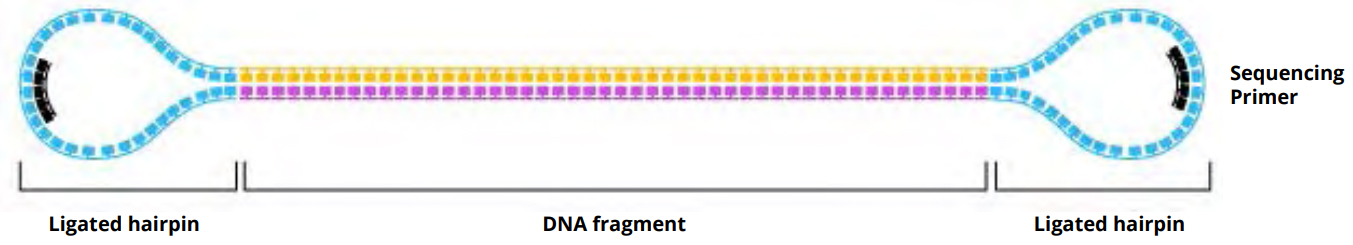
\includegraphics[width=\linewidth, height=0.05\textheight]{Pictures/Smrt_template.jpg}
		\caption{SMRT-bell template}\label{fig:smrtbell}
	\end{subfigure}
	\vspace{20pt}
	\hspace{5em}
	\begin{subfigure}{0.4\linewidth}
		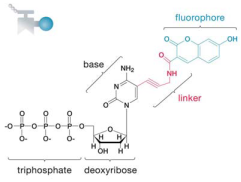
\includegraphics[width=\linewidth, height=0.2\textheight]{Pictures/Phospholinked_nucleotides.png}
		\caption{Phospholinked Nucleotides}\label{fig:Phospholinked_Nucleotides}
	\end{subfigure}
	\vspace{20pt}
	\begin{subfigure}{0.8\linewidth}
		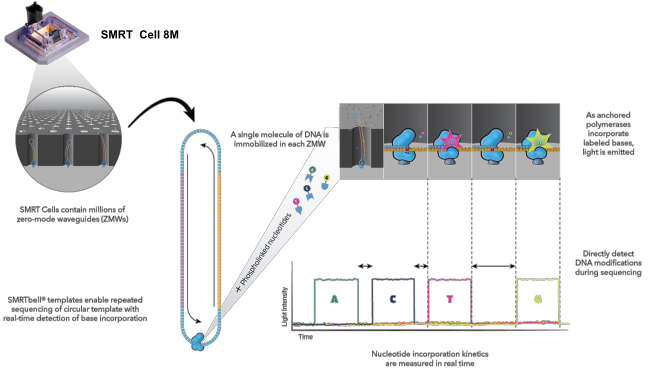
\includegraphics[width=\linewidth, height=0.3\textheight]{Pictures/Mechanism.png}
		\caption{PacBio Single-molecule real time sequencing}\label{fig:mechanism}
	\end{subfigure}
	\captionsetup{width=0.95\textwidth}
	\caption[PacBio SMRT]%
	{\textbf{PacBio SMRT}: At time of writing, PacBio released Sequel II with the provision of an 8M chip, containing 8 million wells, each capable of sequencing one single molecule. Figures adapted from PacBio}
	\label{fig:Mechanism}
\end{figure}
\fi

\subsubsection{Mechanism}
Due to the circular nature of the SMRTbell template, the polymerase is able to continually read through the insert in an interrupted fashion multiple times (or "passes"), resulting in a continuous read (known as polymerase read) (\cref{fig:CCS}). In removing the hairpin-adapters that delineate the repeated insert sequence, this polymerase read is then resolved to multiple reads (known as subreads), which are then further merged to yield one high-quality and highly-accurate consensus read (known as Circular Consensus Sequence - CCS\nomenclature{CCS}{Circular Consensus Sequence}). Dependent on the polymerase lifetime and insert length and, the generation of CCS can increase the accuracy from 85\% (raw subreads) to 99\%, proportional to the number of passes \cite{Travers2010}. 

Consequently, unlike short-reads generated by RNA-Seq, PacBio Iso-Seq reads are not of a set length, but coverage a range of lengths that is dependent on the library size and the polymerase activity\cite{Ardui2018,Rhoads2015}. With previous chemistries, there was a bias towards sequencing molecules of a certain length due to preferential loading of SMRTbell templates - Diffusion Loading favoured shorter molecules\cite{Loomis2013} whereas Magbead Loading allowed proportional loading to the concentration rather than by length, but prevented sequencing of molecules <1kb (discussed in \cref{section:ch2_polbinding_loading}). Previous attempts to mitigate this loading challenge have been to fractionate the library by length (size selection) and enrich for longer cDNA molecules before sequencing\cite{Au2013}, but this approach is more expensive and laborious. Thankfully, recent improvements in both technology and chemistry with usage of molecular crowding agents have alleviated the sequencing read bias and resulting the magbead loading method obsolete \cite{Oikonomopoulos2020}.   


\iffalse
%https://www.pacb.com/wp-content/uploads/2015/09/Guide-Pacific-Biosciences-Template-Preparation-and-Sequencing.pdf
\begin{figure}[h]
	\centering
	\vspace{20pt}
	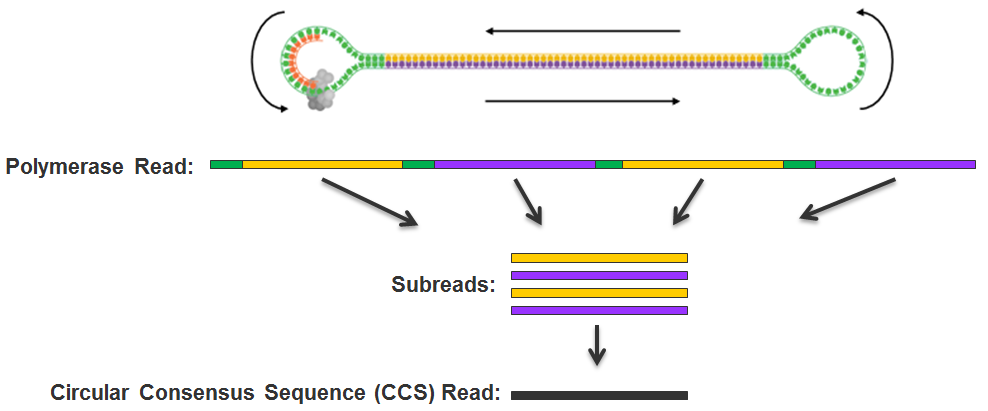
\includegraphics[width=0.8\linewidth, height=0.2\textheight]{Pictures/SMRTAdapter.png}
	\captionsetup{width=0.95\textwidth}
	\caption[Generation of Circular Consensus Sequence]%
	{\textbf{Generation of Circular Consensus Sequence}: CCS is generated by the collapse of multiple subreads, which sequence correspond to the double-stranded cDNA of interest. The greater the number of "passes" sequenced by the polymerase, the longer the polymerase read, the more subreads generated, and subsequently the higher the quality of CCS. Picture adapted from PacBio}
	\label{fig:CCS}
\end{figure}
\fi

\subsubsection{Performance and Run Quality Metric}
Suboptimal sequencing performance could be due to various reasons from potential issues with the instrument and sequencing reagents, to poor library preparation and incorrect loading. Evaluation of the performance of the DNA Internal Control (described in \cref{section:ch2_sequencing}) and productivity metrics would provide useful insights into the performance of a sequencing run. 

\boldheader{DNA Internal Control} 
Sequencing metrics for the DNA Interal Control (described in \cref{section:ch2_sequencing}) include: i) the number of control reads, ii) the mean polymerase read length of the control and iii) the proportion of identity match between the control raw reads and the control reference sequence (concordance). The expected values from a correctly prepared control in a sequencing run, with a 4hr pre-extension time and a 20hr capture time is documented in \cref{tab:control_Isoseqmetrics}. Low control read length and/or low control read counts suggest issues with the PacBio instrument and consumables, whereas expected values indicate sample-specific issues. The corcordance value is a useful metric for optimum loading whereby over-loaded SMRT cells would typically have a lower value (<0.84).

\begin{table}[!h]
	%\captionsetup{justification=raggedright,width=1.45\textwidth}
	\caption[Iso-Seq DNA Internal Control Sequencing Metrics]%
	{\textbf{Iso-Seq DNA Internal Control Sequencing Metrics.} The expected median values for the number of control reads (median count), the control polymerase read length (median length), and the identity match between conrol raw reads and reference sequence (median concordance). The expected values shown are assuming a sequencing run performed with SMRT cells 1M v3 with Sequel DNA Internal Control Complex, Sequel Sequnecing Kit 3.0 on the Sequel I with a 4hr pre-extension time of 4hrs and a 20hr capture time.}
	\label{tab:control_Isoseqmetrics}
	
	\centering
	\begin{tabular}{@{}cccc@{}}
		\toprule
		Metrics         & Median Count (QR)     & Median Length (kb) (QR) & Median Concordance (QR) \\ \midrule
		Expected Values & 6900 (4,000 - 10,200) & 46.9 (41.5 – 52.5) & 0.862 (0.857 – 0.867)   \\ \bottomrule
	\end{tabular}
\end{table}


\boldheader{Productivity Metrics} 
Productivty metrics, or loading metrics, is a measure of the number of ZMWs that have generated a positive signal and subsequently, useful sequencing data. Each ZMW is classified as either: 
\begin{itemize}
	\item P0 (Productivity 0): no active sequencing polymerase complex with no signal 
	\item P1 (Productivity 1): productive ZMWs with a high quality (HQ) region within read 
	\item P2 (Productivity 2): detectable signal but no HQ region detected, possibly due to overloading of multiple inserts with multiple polymerases
\end{itemize}
High quality region is defined as a high quality sequence of >50bases. These metrics are also dependent on chemistry, pre-extension, and movie runtime.  

In general, a good sequencing run has a 20-30\% P0 (proportion of empty ZMWs). A lower P0 (<20\%) from over-loading of polymerase-bound complexes on SMRT cell would result in poorer sequencing yield (noisy base-calling) and shorter P1 polymerase reads; whereas, a higher P0 (>40\%) from under-loading would result in fewer P1 reads and subsequently lower sequencing yield. Of note, a combination of high P0, low P1 and high P2 loading profile indicates presence of contaminants (possibly due to poor AMPure bead purification) that is interferring with productive polymerase activity. A good balance between P0, P1, and P2 is therefore essential and can be achieved by determining an optimum loading concentration through performing titrations of multiple loading concentrations.  	

A good run is defined by 50-70\% P1, a >XX kB polymerase read-length. These metrics are dependent on chemistry, pre-extension, and movie-runtime. 